\chapter{Implementation}
\section{Differences between \ac{CPU} and \ac{GPGPU} hardware}
Before detailing the specific algorithms and configurations used by the RubiCL project, it is necessary to contrast two of the heterogeneous target architectures.

\ac{CPU} and \ac{GPGPU} architectures have diverged significantly due to differing traditional applications.

\ac{CPU} devices have had a long history of optimisation for sequential processing. As such, they have high clock-speeds and integrated hardware designed to increase instruction throughput; Modern processors rely heavily on \emph{branch predictors} and identifying opportunities for speedup via \emph{out-of-order execution}.

Conversely, the graphics pipeline tends to mainly utilise \ac{SIMD} operations. These consist of periods where the same few calculations are applied to vast quantities of data. With this execution pattern, complicated optimising hardware and higher clock-speeds are less favourable. Instead, hardware designers achieve incredible throughput by placing many massively parallel, yet simple, execution units on a single chipset.

In short, common \ac{GPGPU} hardware lacks many optimisations targeting single-threaded performance. More significantly, devices lack the ability to branch by jumping during execution. A flat sequence of instructions is processed by the hardware scheduler. Conditional logic is provided by condition-variable flags set on individual instructions. These masking flags state whether execution of each statement within a branch segment should occur.

The inability to jump causes code that branches to be necessarily inefficient. Any branching logic within a kernel will leave some execution units idling until the code path converges again.

Luckily, \ac{GPGPU} devices compensate by being exceptional at tasks resembling those that they were designed for: \ac{SIMD} computation patterns. A high-end \ac{GPU}, such as the \emph{Radeon R9 290X}, can contain as many as $44$ compute-units. Each compute unit is capable of scheduling $64$ concurrent \ac{SIMD} operations. At full utilisation, this vastly outperforms the raw instruction-rate of any \ac{CPU} device. The amount of parallelism possible in a latest-generation desktop \ac{GPGPU} is simply several orders of magnitude higher.

The goal of this project's implementation phase is to produce an easy-to-use library that presents significant throughput gains to an end-user performing common tasks.

\section{Parallel primitives}
\subsection{Map}
\verb|Map| is a higher-order function that mutates all elements in a provided input vector by applying a function parameter. It can be used to concisely describe a uniform alteration.
\verb|Map| is simple to parallelise since no sharing of each individual thread's state is required.
\paragraph*{Algorithm design}
\begin{algorithm}
  \caption{\emph{Map} higher-order function with sequential execution.}
  \label{alg:seqmap}

  \begin{algorithmic}
    \Function{SeqMap}{$f, A$}
      \ForAll{$a_i \in A$}
        \State{$a_i \Leftarrow$ \Call{$f$}{$a_i$}}
      \EndFor
    \EndFunction
  \end{algorithmic}
\end{algorithm}

Upon examining the sequential implementation of the \verb|map| primitive shown in Algorithm~\ref{alg:seqmap}, it is clear that iteration $i$ only reads and writes value $a_i$.

The dependency graph for a \verb|map| of $\|A\| = 6$ is shown in Figure~\ref{fig:mapgraph}.

\begin{figure}[h]
  \caption{\emph{Map} dependency graph}
  \label{fig:mapgraph}
  \begin{center}
    \begin{tikzpicture}
      [scale=.8,auto=left,every node/.style={circle}]

      \foreach \el/\x/\val in {n1/1/a_1, n2/2/a_2, n3/3/a_3, n4/4/a_4, n5/5/a_5, n6/6/a_6}
        \node (\el) at (2 * \x, 0) {$\val$};

      \foreach \el/\x/\val in {n1/1/a_1, n2/2/a_2, n3/3/a_3, n4/4/a_4, n5/5/a_5, n6/6/a_6}
        \path (\el) edge [anchor=center,loop above] node {} (\el);

    \end{tikzpicture}
  \end{center}
\end{figure}

When analysing data-dependency graphs, such as the one above, any partitioning that doesn't sever edges denotes a valid parallel strategy. Since Figure~\ref{fig:mapgraph} contains no inter-node dependencies, it is trivial to schedule the task concurrently on many compute units. The \verb|map| task is \emph{embarrassingly parallel}.

\algblockdefx[Pf]{PFor}{EndPFor}{\textbf{in parallel, for} }{\textbf{end parallel for}}
\begin{algorithm}
  \caption{\emph{Map} higher-order function with parallel execution.}
  \label{alg:parmap}

  \begin{algorithmic}
    \Function{ParMap}{$f, A$}
      \PFor{$a_i \in A$}
        \State{$a_i \Leftarrow$ \Call{$f$}{$a_i$}}
      \EndPFor
    \EndFunction
  \end{algorithmic}
\end{algorithm}

\paragraph*{Equivalent \ac{OpenCL} kernel design}
The \ac{OpenCL} execution model suggests performing tasks over a dataset by scheduling many distinct work-units. As a result, the side-effects of Algorithm~\ref{alg:parmap}'s loop body are now provided by the result of many individual kernel-function invocations. Algorithm~\ref{alg:oclmap} describes an \ac{OpenCL} kernel that performs \verb|map| computation with a size $\|A\|$ work-group.

\begin{algorithm}
  \caption{\emph{Map} higher-order function in OpenCL kernel form.}
  \label{alg:oclmap}

  \begin{algorithmic}
    \State{$f \Leftarrow$ \Call{MutationFunction}{}}

    \Function{MapKernel}{$A$}
      \State{\Call{DeclareVariables}{$f$}}
      \State{$i \Leftarrow$ \Call{GetGlobalID}{}}
      \State{$a_i \Leftarrow$ \Call{$f$}{$a_i$}}
    \EndFunction
  \end{algorithmic}
\end{algorithm}

\paragraph*{Alternative kernel investigation}
\subparagraph*{Motivation}
After producing a system that performs \verb|map| parallelisation akin to Algorithm~\ref{alg:oclmap}, suspicion arose over whether it was excessive to schedule one work-unit per element. With traditional threaded programming, there is a significant performance cost when creating each parallel subroutine. In addition, with many kernel invocations all writing to offsets in the globally-available $A$, it was theorised that large numbers of competing memory access requests would hamper throughput.

\subparagraph*{Kernel adaption}
In order to ensure that any anticipated scaling issues were avoided, a new kernel design was constructed. The alternate design avoids scheduling a number of work-units greater than the number of compute-units present.

\begin{algorithm}
  \caption{\emph{Map} higher-order function in reduced-work-unit OpenCL kernel form.}
  \label{alg:oclmap2}

  \begin{algorithmic}
    \State{$f \Leftarrow$ \Call{MutationFunction}{}}
    \State{$width \Leftarrow \ceil{\frac{\|A\|}{compute\_units}}$}


    \Function{MapKernel}{$A, width, \|A\|$}
      \State{\Call{DeclareVariables}{$f$}}
      \State{$i \Leftarrow$ \Call{GetGlobalID}{}}
      \State{$i_{initial} \Leftarrow i \times width$}
      \State{$i_{next} \Leftarrow (i + 1) \times width$}
      \For{$i \in ((i_{initial} \ldots (i_{next} - 1) \cap (i_{initial} \ldots (\|A\| - 1))$}
        \State{$a_i \Leftarrow$ \Call{$f$}{$a_i$}}
      \EndFor
    \EndFunction
  \end{algorithmic}
\end{algorithm}

The adapted kernel, now performing \verb|map| computation using a size $\|CU\|$ work-group, is presented in Algorithm~\ref{alg:oclmap2}.

\subparagraph*{Results}
After benchmarking the execution time of the kernels presented in Algorithms \ref{alg:oclmap} and \ref{alg:oclmap2}, no significant difference in performance was found. This suggests that the overhead for work-unit scheduling within the \ac{OpenCL} framework is very low. It also suggests that simultaneous access to neighbouring global-buffer elements does not affect latency worse than strided simultaneous access.

Influenced by these findings, the decision was made to use Algorithm~\ref{alg:oclmap} for \verb|map| tasks. This is due to the design being conceptually simpler, and therefore choosing the most basic solution that works well.

\subsection{Scan}
\verb|Reduce| is a higher-order function that takes an array and an initial `result' value (usually an identity value) and then repeatedly applies a combining function to produce an output.

The final result is equivalent to repeatedly updating the initial value with the output of itself and the next set member using the combiner. Using this technique, the input array is consumed once while the result is cumulatively generated. Any associative reduction function can be parallelised to increase throughput.

A well-known example of reduction is when the initial value is $0$ and the combining function is \verb|+(x, y)|. This results in \emph{summation} of an input dataset.

\verb|Scan| is similar to \verb|Reduce| in that it takes an input vector and a combining function.

Instead of returning the final result, Scan returns a vector that is equal to the intermediate values if the combining function was incrementally applied from one end of the dataset to the other. \verb|Scan| can also exploit a highly-parallel architecture when supplied with suitable operators.

\paragraph*{Algorithm design}
\begin{algorithm}
  \caption{\emph{Inclusive Scan} higher-order function with sequential execution.}
  \label{alg:seqscan}

  \begin{algorithmic}
    \Function{SeqScan}{$f, a_{-1}, A$}
      \ForAll{$a_i \in A$}
      \State{$a_i \Leftarrow$ \Call{$f$}{$a_{i-1} , a_i$}}
      \EndFor
    \EndFunction
  \end{algorithmic}
\end{algorithm}

Unlike sequential \verb|map|, iteration $i$ now reads from both $a_{i-1}$ and $a_{i}$ in addition to writing $a_i$. This produces a data-dependency graph with greater connectedness, shown in Figure~\ref{fig:scangraph}

\begin{figure}[h]
  \caption{\emph{Inclusive Scan} dependency graph}
  \label{fig:scangraph}
  \begin{center}
    \begin{tikzpicture}
      [scale=.8,auto=left,every node/.style={circle}]

      \node (init) at (0, 0) {$initial$};
      \foreach \el/\x/\val in {n1/1/a_1, n2/2/a_2, n3/3/a_3, n4/4/a_4, n5/5/a_5, n6/6/a_6}
        \node (\el) at (2 * \x, 0) {$\val$};


      \foreach \el/\prev in {n1/init, n2/n1, n3/n2, n4/n3, n5/n4, n6/n5} {
        \path (\el) edge [anchor=center,loop above] node {} (\el);
        \draw[->] (\el) -- (\prev);
      }

    \end{tikzpicture}
  \end{center}
\end{figure}

It is clear that no partitioning of this graph exists that does not sever edges. Therefore, this task is not embarrassingly parallel.

However, this does not mean that all hope is lost. It is possible to efficiently parallelise a \verb|scan| task, but it requires performing computation split over multiple \emph{stages}. One method for achieving this is demonstrated in Figure~\ref{fig:odd_even}.

\begin{figure}[h]
\begin{center}
  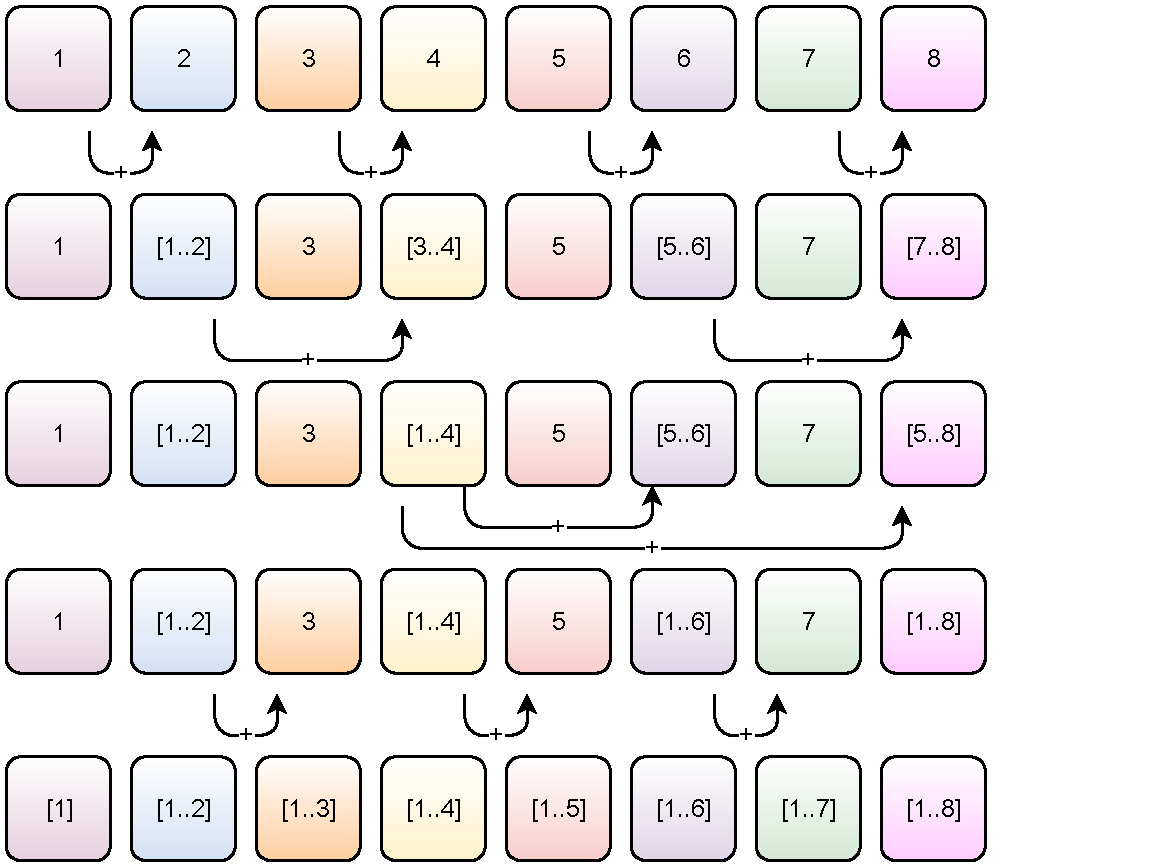
\includegraphics[width=0.8\textwidth]{./figures/oddeven.pdf}
  \caption{An example of parallelised \emph{inclusive scan} using the \emph{odd-even} algorithm, detailed in Algorithm~\ref{alg:parscan}}
  \label{fig:odd_even}
\end{center}
\end{figure}

\begin{algorithm}
  \caption{Odd-even style \emph{Scan} higher-order function with parallel execution.}
  \label{alg:parscan}

  \begin{algorithmic}
    \Function{ParScan}{$f, A$}
      \State{$level \Leftarrow 2$}

      \While{$level <= \|A\|$}
        \PFor{$l \in (level\ldots2 \times level\ldots\|A\|)$}
          \State{$A_l \Leftarrow$ \Call{$f$}{$A_l, A_{l - \frac{level}{2}}$}}
        \EndPFor
        \State{$level \Leftarrow 2 \times level$}
      \EndWhile

      \If{$level = \|A\|$}
      \State{$level \Leftarrow \frac{level}{2}$}
      \EndIf

      \While{$level > 1$}
      \PFor{$l \in (level + \frac{level}{2}\ldots2 \times level + \frac{level}{2}\ldots\|A\|)$}
          \State{$A_l \Leftarrow$ \Call{$f$}{$A_l, A_{l - \frac{level}{2}}$}}
        \EndPFor
        \State{$level \Leftarrow \frac{level}{2}$}
      \EndWhile

    \EndFunction
  \end{algorithmic}
\end{algorithm}

A parallel algorithm's \emph{cost} is defined as its asymptotic runtime multiplied by the required number of compute-units.


The \emph{odd-even} prefix sum algorithm can process a dataset of size $n$ in $O(\log n) + \frac{O(n)}{\|CU\|}$ stages of execution. This gives a cost of $O(\|CU\| \log n) + O(n)$.
Importantly, it is \emph{cost-optimal}, meaning that its cost is equal to that of the best-known sequential algorithm, when $\|CU\| = O(\frac{n}{\log n})$. This is an entirely reasonable assumption given large datasets and the number of compute-units ($4-48$) present on commodity \ac{OpenCL} devices.

This discovery suggests that it is possible to increase the throughput of \verb|scan| tasks significantly, by scheduling them across massively parallel \ac{OpenCL} devices.

\paragraph*{\ac{OpenCL} kernel design}
In fact, the kernel and calling algorithm utilised differs from \emph{odd-even} scan in that it is designed to perform better on typical \ac{OpenCL} compute devices.

It was adapted from an example provided within the Apple \ac{OpenCL} SDK, modified to allow arbitrary element types and operate on buffers within the RubiCL environment.
\todo{Explain bank conflicts and mitigating their effects?}

\subsection{Scatter}
The \verb|Scatter| primitives receives an input array $A$, an array of indices $I$, and an output array $B$. It updates $B$ such that $B_{I_i} \Leftarrow A_i$. Put otherwise, it inserts the value given at offset $i$ of $A$ into $B$, at the position given by the value at offset $i$ of $I$.

\verb|Scatter| is useful for reordering a collection or projecting a subset of an input dataset into an output dataset.

\begin{algorithm}
  \caption{\emph{Scatter} primitive with sequential execution.}
  \label{alg:seqscatter}

  \begin{algorithmic}
    \Function{SeqScatter}{$A, I, B$}
      \ForAll{$a_i \in A$}
      \State{$B_{I_i} \Leftarrow A_i$}
      \EndFor
    \EndFunction
  \end{algorithmic}
\end{algorithm}

\paragraph*{Permutation scatter}
It is important to draw attention to an important distinction in types of \verb|scatter| operation. \emph{Permutation Scatter} is defined as a scatter operation where all $i \in I$ are unique. Therefore, there are no two writes to the same destination in $B$. Other forms of \verb|scatter| increase complexity, as rules that state how to handle write collisions within the transaction must be introduced.

Luckily, for this project's needs we only need to analyse the simpler \emph{permutation scatter}. We can assume that no two writes to the same destination offset will occur.

\begin{figure}[h]
  \caption{\emph{Permutation Scatter} dependency graph}
  \label{fig:scatgraph1}
  \begin{center}
    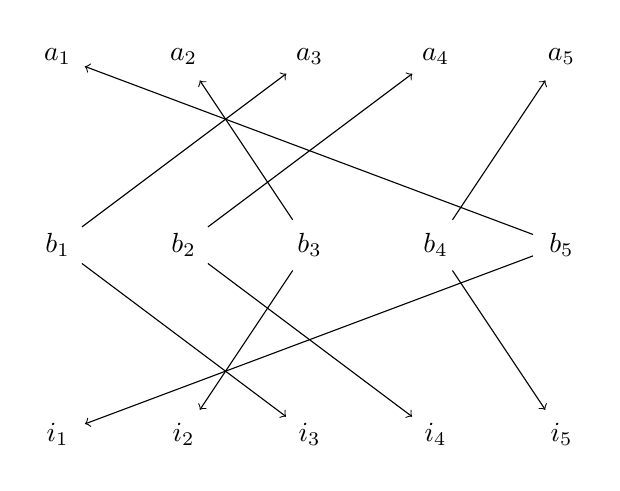
\begin{tikzpicture}
      [scale=.8,auto=left,every node/.style={circle}]

      \foreach \x in {1, 2, 3, 4, 5} {
        \node (a\x) at (2 * \x, 3) {$a_{\x}$};
        \node (b\x) at (2 * \x, 0) {$b_{\x}$};
        \node (i\x) at (2 * \x, -3){$i_{\x}$};
      }

      \foreach \s/\d in {1/5, 2/3, 3/1, 4/2, 5/4}{
        \draw[->] (b\d) -- (a\s);
        \draw[->] (b\d) -- (i\s);
      }

    \end{tikzpicture}
  \end{center}
\end{figure}
A data-dependency graph for a typical scatter operation is shown in Figure~\ref{fig:scatgraph1}.
At first, it may appear complicated. However, when nodes $b_i \in B$ are reordered by their data-source, a valid partitioning becomes clear. The result of this simplification is shown in Figure~\ref{fig:scatgraph2}.

\begin{figure}[h]
  \caption{\emph{Permutation Scatter} dependency graph, simplified.}
  \label{fig:scatgraph2}
  \begin{center}
    \begin{tikzpicture}
      [scale=.8,auto=left,every node/.style={circle}]

      \foreach \s/\d in {1/5, 2/3, 3/1, 4/2, 5/4}{
        \node (a\s) at (2 * \s, 2) {$a_{\s}$};
        \node (b\d) at (2 * \s, 0) {$b_{\d}$};
        \node (i\s) at (2 * \s, -2){$i_{\s}$};
        \draw[->] (b\d) -- (a\s);
        \draw[->] (b\d) -- (i\s);
      }
    \end{tikzpicture}
  \end{center}
\end{figure}

This suggests that \verb|scatter|, when using unique indices, is \emph{embarrassingly parallel}. Like \verb|map|, this produces an easy-to-understand parallel conversion, shown in Algorithm~\ref{alg:parscatter}.

\begin{algorithm}
  \caption{\emph{Permutation Scatter} primitive with parallel execution.}
  \label{alg:parscatter}

  \begin{algorithmic}
    \Function{ParScatter}{$A, I, B$}
      \PFor{$a_i \in A$}
      \State{$B_{I_i} \Leftarrow A_i$}
      \EndPFor
    \EndFunction
  \end{algorithmic}
\end{algorithm}

\paragraph*{Equivalent \ac{OpenCL} kernel design}
\begin{algorithm}
  \caption{\emph{Permutation Scatter} primitive in \ac{OpenCL} kernel form.}
  \label{alg:scatterkernel}
  \begin{algorithmic}
    \Function{ScatterKernel}{$A, I, B$}
      \State{$i \Leftarrow$ \Call{GetGlobalID}{}}
      \State{$B_{I_i} \Leftarrow A_i$}
    \EndFunction
  \end{algorithmic}
\end{algorithm}

The kernel design is simpler than that of \verb|map|, since function side-effects do not need to be included. It is presented in Algorithm~\ref{alg:scatterkernel}.

\subsection{Filter}
\verb|filter| is a higher-order function that applies a predicate function on elements of a dataset. It returns the subset of the input vector for which the predicate evaluates true. 

A sequential implementation of the primitive is shown in Algorithm~\ref{alg:seqfilter}.

\begin{algorithm}
  \caption{\emph{Filter} higher-order function with sequential execution.}
  \label{alg:seqfilter}

  \begin{algorithmic}
    \Function{SeqFilter}{$A, predicate$}
      \State{$Result \Leftarrow$ \verb|[ ]|}
      \ForAll{$a_i \in A$}
      \If{\Call{$predicate$}{$a_i$}}
      \State{\Call{Push}{$Result, a_i$}}
      \EndIf
      \EndFor
      \State{$A \Leftarrow Result$}
    \EndFunction
  \end{algorithmic}
\end{algorithm}

Checking the predicate is simple to do in parallel, since whether to keep each element depends only on the value of that element. However, producing and returning the subset is significantly more involved. Complication stems from the position of each kept item in the output array depending on the state of previous elements in the input vector.

\begin{figure}[h]
  \caption{\emph{Filter} dependency graph.}
  \label{fig:filtergraph}
  \begin{center}
    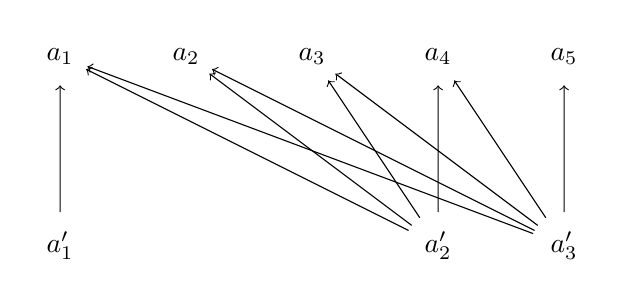
\begin{tikzpicture}
      [scale=.8,auto=left,every node/.style={circle}]

      \foreach \x in {1, 2, 3, 4, 5}{
        \node (a\x) at (2 * \x, 3) {$a_{\x}$};
      }

      \foreach \x/\y in {1/1, 4/2, 5/3}{
        \node (b\x) at (2 * \x, 0) {$a^\prime_{\y}$};
      }

      \draw[->] (b1) -- (a1);

      \draw[->] (b4) -- (a1);
      \draw[->] (b4) -- (a2);
      \draw[->] (b4) -- (a3);
      \draw[->] (b4) -- (a4);


      \draw[->] (b5) -- (a1);
      \draw[->] (b5) -- (a2);
      \draw[->] (b5) -- (a3);
      \draw[->] (b5) -- (a4);
      \draw[->] (b5) -- (a5);
    \end{tikzpicture}
  \end{center}
\end{figure}

The \verb|filter| operation is clearly not \emph{embarrassingly parallel}. However, there is no need to search for an involved parallel algorithm. We can construct an efficient \verb|filter| operation by reusing the previously defined parallel primitives, \verb|map|, \verb|scan|, and \verb|scatter|. This insight transforms a hard problem into one much easier to solve.

\paragraph*{Composing a parallel solution}
The first stage of producing a parallel \verb|filter| primitive is recognising the distinct data dependencies:
\begin{enumerate}
  \item Whether an element is kept.
  \item Where any kept element appears in the result.
  \item The total number of elements kept, since we cannot dynamically allocate memory.
\end{enumerate}

\subparagraph*{Identifying kept elements}
The information required by dependency $1$ can be obtained by performing a \verb|map| task on the dataset using the predicate function. The sole difference is that the result should be stored in a new buffer instead of overwriting the previous value.

Assuming we have an input vector $A$ and a newly created predicate buffer $P$, we now know that any $A_i$ should be kept if, and only if, $P_i$.

\subparagraph*{Knowing where to place kept elements}
Once we have produced a predicate buffer, via $1$, we can easily derive the destination of kept elements ($2$). If the predicate buffer is stored as a vector of bit-flags, the number of kept elements at point $P_i$ is equal to element $i$ of the prefix-summation of $P$. This connection is illustrated in Figure~\ref{fig:wheretoplace}

\begin{figure}[h]
\begin{center}
  \caption{Using prefix-sum to determine insertion points.}
  \label{fig:wheretoplace}

  $predicate$ = \verb|keep_if_even|
  \vskip 10pt
  \begin{tabular}{ | c | c | c | c | c | c |}
    \hline
    Input dataset   & 0 & 1 & 2 & 3 & 4 \\ \hline
    Presence buffer & 1 & 0 & 1 & 0 & 1 \\ \hline
    Prefix sum      & 1 & 1 & 2 & 2 & 3 \\ \hline
    Insertion point & 0 & - & 1 & - & 2 \\ \hline
  \end{tabular}
\end{center}
\end{figure}

The translation from prefix-summed buffer element to insertion point is just an off-by-one adjustment.
Furthermore, since \verb|map| followed by \verb|scan| is cost $O(n) + O(n) = O(n)$, we can obtain these insertion points \emph{cost-optimally}.

\subparagraph*{Counting the number of kept elements}
Following the calculation of dependencies $1$ and $2$, obtaining $3$ is trivial. It is simply the final element of the prefix-sum buffer. This can be retrieved by a single lookup after the other sub-problems have been solved.

\paragraph*{Complete solution}
By utilising \verb|map|, \verb|scan|, and a conditional-modified \verb|scatter|, \verb|filter| can be performed with cost $O(n) + O(n) + O(1) + O(n) = O(n)$. This is identical to the sequential algorithm presented earlier and is therefore \emph{cost-optimal}. Again, this suggests that \verb|filter| tasks can benefit from increased throughput when scheduled across multiple compute-units.

The combined process is demonstrated in Algorithm~\ref{alg:parfilter}.

\begin{algorithm}
  \caption{\emph{Filter} higher-order function with parallel execution, composed from other primitives.}
  \label{alg:parfilter}

  \begin{algorithmic}
    \Function{ParFilter}{$A, p$}
    \State{$P \Leftarrow$ \Call{ParMap}{$A, p$}}
    \State{$I \Leftarrow$ \Call{ParScan}{$P, +$}}
    \State{$B \Leftarrow$ \Call{Zeros}{$I_{\|I\|}$}}
    \PFor{$a_i \in A$}
      \If{$P_i$}
        \State{$B_{I_i - 1} \Leftarrow A_i$}
      \EndIf
    \EndPFor
    \State{$A \Leftarrow B$}
    \EndFunction
  \end{algorithmic}
\end{algorithm}

The parallel loop body is a modified version of the \verb|scatter| task. The divergence is that it only performs scattering if the predicate element is set.

\subsection{Count}
The \verb|count| function is very similar to the aforementioned \verb|filter| primitive.
Instead of returning the subset of a dataset that passes a predicate, it returns how many times the predicate was passed.

To avoid writing extra code providing counting functionality, we can re-use many components of the \verb|filter| implementation. Namely, the \verb|map| task that sets predicate bits for each element, followed by the \verb|scan| task to yield the number of kept elements. Reduction can be performed in  less work than a \verb|scan| primitive, as the intermediate values are not required. However it is asymptotically identical, therefore the \verb|scan| primitive can be reused to reduce developer workload.
Further work can include replacing this suboptimal lack of specialisation with a faster reduction task.


\subsection{Sort}
\todo{Explain bitonic sort}


\section{Management System}

\subsection{Converting between Ruby and C objects}
One important issue to overcome when designing an library to accelerate Ruby processing, is the fact that the RubyVM stores all values within \emph{objects}, in a manner that is very different from C.

Internally, the RubyVM's C implementation references all objects as of type \verb|VALUE|. This value-type is a slight misnomer as it (usually) contains a pointer to an object structure.

There are several object structures used to represent raw data within the RubyVM. However they all fall into one of two categories:
\begin{itemize}
     \item \verb|RObject| for storing the state of any bespoke object. This includes storage of instance variables and a pointer to the corresponding class hierarchy for lookup of all methods defined.
     \item A specialised object representation, used to increase performance of heavily utilised object types. Examples include \verb|RString|, \verb|RFloat|, and \verb|RArray|.
\end{itemize}

The first member of both structures is another structure called \verb|RBasic|. This contains meta-data about the object, such as what type it is. Therefore, it is possible to obtain the typing information of object designated by a \verb|VALUE|, by examining the meta-data present in it's first structure member.

Since integers are often heavily utilised within computer programs, and often short-lived, the RubyVM implementation avoids the creation of integer objects in order to improve performance.
Instead, it encodes the value of the first $2^{64 - 2}$ integers directly into the \verb|VALUE| `pointer', setting the final 2 bits as the flag \verb|0x01|.
It can be deduced that a pointer with an odd value is not pointing to a valid memory location, as is true for any pointer that does not align to word-length boundaries. In this case, a flag lookup table can be used in order to determine the correct typing information.

When dealing with tagged-pointers, the corresponding value of pointer \verb|p| can be retrieved with \verb|p >> 1|. To create a tagged-pointer, the value \verb|x| can be encoded with \verb?(x << 1) | 0x01 ?. The RubiCL project utilises this fact by transferring an array of \verb|VALUE| pointers directly to the compute-device, whenever annotation has suggested that all contained elements are of \verb|Fixnum| type. There, the bit-shifting conversions, present at either end of the computation pipeline, can be performed in parallel to increase throughput.

\subsection{Transferring data to and from device}
As \ac{OpenCL} is designed to provide an abstraction over specific hardware details, the memory management functionality it provides reflects this agnosticism.
A common method for providing input data to a compute-device is to explicitly create a buffer of the required size, within the device's \emph{context}, and then enqueue a \verb|clWriteBuffer| task to fill it with any elements to process. This buffer object is then provided as a kernel parameter, prior to kernel invocation. To retrieve the processed elements, a \verb|clReadBuffer| task is enqueued.

This workflow causes several issues. Firstly, when the compute-device selected is the system \ac{CPU}, unnecessary data copying occurs. The original location of the dataset is already addressable by the \ac{CPU} device so there is no need to move elements into a new buffer, this just causes unnecessary delay. The same is true when retrieving processed elements, there is no reason that the host program cannot access the element buffer directly. Secondly, when writing data into the device buffer, data-flow occurs through the host device. This is inefficient on many systems when interfacing with a \ac{GPU} device, since \emph{kernel-mode} execution is required to transfer data over the \ac{PCI} bus and \ac{OS}-enforced context switching increases latency.

Luckily, the \ac{OpenCL} \ac{API} provides a solution that is better-suited to the project's data transfer needs.
\emph{Pinned} buffers can be created by specifying the \verb|USE_HOST_PTR| flag and providing a pointer to the dataset residing within host memory.
When a dataset is pinned, the returned buffer object now merely references the original data location, yet can still be provided as a kernel parameter.
Upon providing a pinned buffer parameter, behaviour of the \ac{OpenCL} execution environment is dependent on the target device.
When the kernel is scheduled for execution on the \ac{CPU}, no memory transfer occurs and the original data can be accessed through the reference provided within a pinned buffer.
When the kernel is scheduled for execution on an external device, such as a \ac{GPU}, \ac{DMA} transfer of the dataset occurs and the elements are placed in device-local memory.
Before the host program can access the results of kernel execution, the pinned buffer must be \emph{unmapped}. At this point is it now guaranteed that the host memory state will reflect the finishing state of compute-device computation.

By utilising pinned memory, the RubiCL library avoids any unnecessary copying of data when executing on \ac{CPU} compute-devices. In addition, \ac{GPU} latency is reduced as \ac{DMA} transfer of the required dataset does not cause the \ac{OS} to invoke costly context-switching.

\subsection{Function parser}
The system's function parser is responsible for converting a supplied anonymous function into C syntax. The functionality of the parser is demonstrated in Listing~\ref{lst:parser_ex}
\begin{lstlisting}[
  language=Ruby,
  label=lst:parser_ex,
  caption=The \emph{LambdaBytecodeParser} converts an anonymous function Ruby object into an array of C expressions.
]
foo = 3
a_function = ->(x){ foo * (2 + x) }
#=> #<Proc:0x007f976207ff48@(pry):12 (lambda)>

parser = RubiCL::LambdaBytecodeParser.new(a_function)
#=> #<struct RubiCL::LambdaBytecodeParser
#   function=#<Proc:0x007f9761c362c0@(pry):15 (lambda)>>

parser.bytecode
#=> " == disasm: <RubyVM::InstructionSequence:block in __pry__
# == catch table
# | catch type: redo   st: 0000 ed: 0016 sp: 0000 cont: 0000
# | catch type: next   st: 0000 ed: 0016 sp: 0000 cont: 0016
# |-----------------------------------------------------------
# local table (size: 2, argc: 1 [opts: 0, rest: -1, post: 0,
#                                  block: -1, keyword: 0@3] s3)
#   [ 2] x<Arg>     
#   0000 trace            256                            (  22)
#   0002 trace            1
#   0004 getlocal         foo, 2
#   0007 trace            1
#   0009 putobject        2
#   0011 getlocal_OP__WC__0 2
#   0013 opt_plus         <callinfo!mid:+, argc:1, ARGS_SKIP>
#   0015 opt_mult         <callinfo!mid:*, argc:1, ARGS_SKIP>
#   0017 trace            512
#   0019 leave"
parser.parsed_operations
#=> [3, 2, "x", "+", "*"]

parser.to_infix
#=> ["3 * (2 + x)"]
\end{lstlisting}

The conversion process occurs over three stages: dumping bytecode, lexing, and reconstruction.

\paragraph*{Obtaining function bytecode}
The bytecode instructions, produced by a compiled anonymous function object, are provided by the \verb|RubyVM::InstructionSequence| module's \verb|disassemble| method.
It returns a human readable string that includes all stack-machine instructions.

\paragraph*{Lexing bytecode string}
Instructions of interest are extracted from the human-readable string. This is achieved via a regular expression containing a whitelist of keywords:
\begin{verbatim}
/(?:\d*\s*(?:(getlocal.*|putobject.*|opt_.*|branch.*).?))/
\end{verbatim}

The instructions are then tokenised, by the process detailed in Listing~\ref{lst:tokeniser_rules}.
The end result is a list of tokens representing stack-machine instructions, in \ac{RPN}.

The heavy reliance on regular expressions to parse bytecode is inelegant and fragile.
However, with access only to a human-readable string, and a lack of any formal grammar, it was the best tool at hand to get the job done.

\begin{lstlisting}[
  language=Ruby,
  label=lst:tokeniser_rules,
  caption=Tokenisation rules for lexing human-readable bytecode.
]
def translate(operation)
  case operation
  # First function argument
  when /getlocal_OP__WC__0 #{function.arity + 1}/
    'x'
  # Second function argument
  when /getlocal_OP__WC__0 #{function.arity}/
    'y'
  # Indexed bound variable
  when /getlocal_OP__WC__1 \d+/
    id = /WC__1 (?<i>\d+)/.match(operation)[:i].to_i
    index = locals_table.length - (id - 1)
    beta_reduction locals_table[index]
  # Named bound variable
  when /getlocal\s+\w+,\s\d+/
    name = /getlocal\s+(?<name>\w+),/.match(operation)[:name].to_sym
    beta_reduction name
  # Literal Zero
  when /putobject_OP_INT2FIX_O_0_C_/
    0
  # Literal One
  when /putobject_OP_INT2FIX_O_1_C_/
    1
  # Floating-Point Literal
  when /putobject\s+-?\d+\.\d+/
    operation.split(' ').last.to_f
  # Integer Literal
  when /putobject\s+-?\d+/
    operation.split(' ').last.to_i
  # Method Sending
  when /opt_send_simple/
    /mid:(?<method>.*?),/.match(operation)[:method].to_sym
  # Conditionals
  when /branch/
    LOOKUP_TABLE.fetch operation[/branch\w+/].to_sym
  # Built-in Operator
  when /opt_/
    LOOKUP_TABLE.fetch operation[/opt_\w+/].to_sym
  else
    raise "Could not parse: #{operation} in #{bytecode}"
  end
end

def beta_reduction variable_name
  function.binding.local_variable_get variable_name
end
\end{lstlisting}

\paragraph*{Expression reconstruction}

\begin{algorithm}[h]
  \caption{\ac{RPN} to infix expression conversion.}
  \label{alg:to_infix}

  \begin{algorithmic}
    \Function{RpnToInfix}{$tokens$}
    \State{$Stack \Leftarrow$ \verb|[ ]|}
    \While{\Call{length}{$tokens$} $ > 0$}
    \State{$token \Leftarrow $\Call{shift}{$tokens$}}
    \If{\Call{isLiteral}{$token$}}
    \State{\Call{push}{$Stack, token$}}
    \Else
    \State{$right \Leftarrow $\Call{pop}{$Stack$}}
    \State{$left \Leftarrow $\Call{pop}{$Stack$}}
    \State{$combined \Leftarrow $\Call{combine}{$token, left, right$}}
    \State{\Call{push}{$Stack, combined$}}
    \EndIf
    \EndWhile
    \EndFunction
  \end{algorithmic}
\end{algorithm}

The final stage of the translation process. It requires converting \ac{RPN} to infix form.
There is a well-defined algorithm for doing so, provided in Algorithm~\ref{alg:to_infix}.

The conversion algorithm makes the assumption that all non-literals are functions with arity 2. This is justified since it covers all mathematical operators required by the library. Outliers include unary negation and method sending operations. These are detected and handled by an additional level of logic, omitted from the basic algorithm for brevity.

\paragraph*{Handling conditionals}
Conditional operators, such as \verb|&&|, complicate the reconstruction process. Instead of modifying the value of a stack-machine, they may perform a branch. Whether or not this occurs depends on the \verb|truthyness| of the current value. This is caused by the optimisation of short-circuiting boolean calculations.

Luckily, at the point that the branch is possibly triggered, no mathematical operators will mutate the previous value directly. This means that the difficultly of handling branching can be sidestepped by simply abandoning the current expression, ending in a conditional, and starting a new stack. All expressions produced are then just combined in order after the token stream has been exhausted.

\subsection{Task queue}
The \verb|TaskQueue| management system buffers all deferred tasks, scheduled during the computation pipeline. It is responsible for detecting potential optimisations and applying them prior to dispatch.
By fusing compatible tasks, the number of passes over the data required can be reduced. The rules utilised to select and process tasks eligible for fusion are detailed in Listing~\ref{lst:fusion_rules}.

In the order presented, the types of fusion supported are as follows:
\begin{description}
\item[Map-map fusion] Adjacent \verb|map| tasks can be replaced by a single task that performs the side-effects of both tasks combined.

\item[Filter-filter fusion] Adjacent \verb|filter| tasks can be replaced by a single task that only retains elements that pass both predicates.

\item[Map-filter fusion] A \verb|filter| task following a \verb|map| task can replace it, performing its mutation before generating presence flags. Filter tasks that have gained the additional responsibility to mutate are hereafter referred to as \verb|mapfilter| tasks.

\item[Filter-map fusion] Similarly, a \verb|map| task following a \verb|filter| task should not necessarily be scheduled. The side-effects of the \verb|map| can be performed after filtering by a fused \verb|mapfilter| kernel. This has the disadvantage that branching in the following map task, to avoid unnecessary calculation on items that won't be kept, will cause inefficient stalling in execution. However, if enough work-units are scheduled, the \ac{OpenCL} runtime can identify non-stalled units to swap-in. Nonetheless, time wasted by stalls in a fused kernel is insignificant compared to the time to schedule a new kernel and pass over the data again in a separate \verb|map| task.

\item[Map-mapfilter fusion] No different to \verb|map-filter| fusion. The side-effects of the replaced \verb|map| task are prepended to the \verb|mapfilter|'s preprocessing actions.

\item[Mapfilter-map fusion] Again, advantageous as it avoids scheduling another pass over the data. The side-effects of the unnecessary \verb|map| are appended to the \verb|mapfilter|'s post-processing actions.

\item[Mapfilter-filter fusion] In \verb|mapfilter| tasks that have no post-processing actions, the \verb|filter| segment can be updated in the same manner as \verb|filter-filter| fusion.
\end{description}

\begin{lstlisting}[
  language=Ruby,
  label=lst:fusion_rules,
  caption=Fusion rules for combining tasks within the \emph{TaskQueue}.
]
@tasks = @tasks.reduce [] do |queue, task|
  if (*fixed_queue, previous = queue).empty? then [task]
  else
    case [previous.class, task.class]
    when ([RubiCL::Map] * 2), ([RubiCL::Filter] * 2)
      fixed_queue << previous.fuse!(task)

    when [RubiCL::Map, RubiCL::Filter]
      fixed_queue << RubiCL::MappingFilter.new(
          pre_map: previous, filter: task)

    when [RubiCL::Filter, RubiCL::Map]
      fixed_queue << RubiCL::MappingFilter.new(
          filter: previous, post_map: task)

    when [RubiCL::Map, RubiCL::MappingFilter]
      fixed_queue << task.pre_fuse!(previous)

    when [RubiCL::MappingFilter, RubiCL::Map]
      fixed_queue << previous.post_fuse!(task)

    when [RubiCL::MappingFilter, RubiCL::Filter]
      if previous.has_post_map?
        fixed_queue << previous << task
      else
        fixed_queue << previous.filter_fuse!(task)
      end
    else
      fixed_queue << previous << task
    end
  end
end
\end{lstlisting}

Options to turn-off \verb|TaskQueue| optimisation were introduced so that the magnitude of benefits can be studied. This will be revisited in the \emph{Evaluation} chapter.


\section{Functionality Testing}
A performant system for calculation parallelisation isn't much use if its behaviour is incorrect. In order to increase confidence that the system performs as expected, the library was developed alongside a comprehensive test suite.

Having significant tests around behaviour enables more intrusive alterations to occur smoothly. This allowed the pace of experimentation to increase. New ideas can be verified as resultant in enhanced performance, without introducing behaviour regressions.

The \verb|RSpec|\cite{rspec} testing library was used to produce test-cases. It presents a \ac{DSL} for defining the intended behaviour of objects.

By describing a context corresponding to each feature that an subcomponent is designed to present, and testing boundary cases within that context, a rigid specification of correct behaviour was defined.

The advantages of testing were significant in terms of effort-economy. With a full test-suite execution taking less than $100$ms on the development laptop, it was responsive enough to be triggered by each updated file within the development directory. This immediately highlighted interface clashes and regressions introduced during development. In addition, it reduced the amount of time wasted, manually checking that the system performed as advertised.

Compared to the stressful development practices of other projects witnessed, this development style is subjectively judged to be a significant success of the project.


\section{Performance testing}
A stated goal of the project refers to ``improving dynamic language performance''.
Therefore, it is important that the project provides a method for producing meaningful metrics.
In order to facilitate measurement, a benchmarking suite for easy graph creation was developed.
In addition, an execution mode that displays timing information alongside results was added to the \verb|Logger|.

\subsection{Custom benchmarking environment}
During the lifetime of the project, a benchmarking library was created. It was originally designed as personal project, but was utilised heavily during development of the library.  The benchmark library eases the production of graphs that plot function runtime over a range of input sizes.

A user provides several parameters to the library:
\begin{itemize}
\item A name for the graph.
\item The number of iterations to average benchmark results over.
\item Several function descriptions to test.
\end{itemize}

Each function description also contains parameters:
\begin{itemize}
\item A description of what is being benchmarked.
\item An \verb|Enumerable| providing seeds to the benchmark environment.
\item A function that turns each seed into a \emph{input}. This could be any value, given to the benchmarked function, that responds to \verb|size|.
\item The function to benchmark.
\end{itemize}

The benchmarking environment was used to produce Figure~\ref{fig:ruby_vs_c}, shown earlier in the \emph{Overview} chapter. The code used to generate the graph is shown in Listing~\ref{lst:vs_c_graph}.

\begin{lstlisting}[
  language=Ruby,
  label=lst:vs_c_graph,
  caption=The \emph{asymptotic} library used to generate quick benchmark graphs.
]
require 'asymptotic'
require 'ostruct'

seeds = (20..25)

ruby_input = {
  input_seeds: seeds,
  input_function: ->(seed){ (1..2**seed).to_a }
}

command_line_input = {
  input_seeds: seeds,
  input_function: ->(seed){
    OpenStruct.new.tap { |s| s.size = 2**seed }
  }
}

Asymptotic::Graph.plot(5, "squaring integers and filtering evens",
  "Ruby: Enumerable#map and Enumerable#filter" => {
    function: ->(array){
      array.map { |x| x * x }.select { |x| x % 2 == 0 } 
    },
  }.merge(ruby_input),

  "C: loop for mapping followed by loop for filtering" => {
    function: ->(struct){ `./just_c.o #{struct.size}` },
  }.merge(command_line_input),
)
\end{lstlisting}

The library handles generating an average runtime, using the specified number of test iterations, for each $(function, \|input\|)$ pair.
The garbage collector is turned off for the duration of each test and manual sweeping is triggered after each measurement is taken.
A graph is then produced, using the \verb|gnuplot| library, that compares the performance of all provided functions.

The ability to effortlessly create runtime graphs, for arbitrary given functions, proved useful during experimental development.
When changes were introduced into the codebase, corresponding feature flags were added to the configuration module.
Then, the benchmark environment was be used to plot the performance of the feature turned off against the performance with the feature enabled.
This made it easy to highlight changes in design that altered performance for a given task over a variety of input sizes.

\subsection{Segmented timing information from execution environment}
Overall execution time is an important metric. However, it is helpful to be able to tell what proportion of time is spend doing various tasks during runtime.

In order to achieve this, code that gathers timing information was introduced to the library's native extensions that interact with hardware devices.

With each action triggered by the system, the resultant transaction time was measured.
The low-level code, handling device management, obtained measurements via observing the start and stop time of \ac{OpenCL} library functions.
This data could then be retrieved by the library and inspected to determine the duration of subtasks, transferring or processing data.

Execution duration measurements are taken by native interaction modules, and observed by the management system.
To make these readings available, configuration flags were added to the \verb|Logger| stating that this data should be displayed during runtime.

An example of the finer granularity timing information presented is given in Listing~\ref{lst:segment_times}.
\begin{lstlisting}[
  language=Ruby,
  label=lst:segment_times,
  caption=Segment times presented during command execution.
]
RubiCL::Logger.show_timing_info = true
#=> true

(1..10)[Int].map { |x| x + 100 }.filter { |y| y.even? }[Fixnum]
#> Pipeline Started
#> Pinned Integer Range in 0.039 ms
#> Enqueued
#>  (rubiclmappingfilter5 =>
#>    [
#>      "x = x >> 1", "x = x + 100",
#>      "?{(x % 2 == 0)}?", "x = (x << 1) | 0x01"
#>     ]
#>  )
#> in 3.175 ms
#> Waiting for in-progress tasks took 0.004 ms
#> Retrieved 5 Integers in 0.017 ms
#> Pipeline Complete in 5.109 ms
#=> [102, 104, 106, 108, 110]

\end{lstlisting}


